\esSezione{Cronometro}\label{sec:esercizio5-1}

\begin{traccia}
Progettare, implementare in VHDL e testare mediante simulazione un cronometro, in grado di scandire secondi, minuti e ore a partire da una base dei tempi prefissata (es.\ si consideri il clock a disposizione sulla board). Il progetto deve prevedere la possibilità di inizializzare il cronometro con un valore iniziale, sempre espresso in termini di ore, minuti e secondi, mediante un opportuno ingresso di set, e deve prevedere un ingresso di reset per azzerare il tempo. Il componente deve essere realizzato utilizzando un approccio strutturale, collegando opportunamente dei contatori secondo uno schema a scelta.
\end{traccia}

\progetto

Il cronometro è ottenuto dalla cascata di quattro istanze dello stesso componente, il contatore modulare \texttt{counter\_mod}, che verrà riutilizzato anche negli esercizi successivi. La prima istanza, il prescaler, ha modulo \texttt{F\_CLK}, pari al numero di cicli di clock contenuti in un secondo, e produce un impulso \texttt{tick} una volta al secondo. Fa quindi da divisore di frequenza. Il conteggio dei secondi è comunque pilotato da un segnale di abilitazione, così tutto il circuito resta sincrono con il clock della board.

Le tre istanze successive contano i secondi (modulo 60, 6 bit), i minuti (modulo 60, 6 bit) e le ore (modulo 24, 5 bit). L'uscita di riporto \texttt{tc} di ciascun contatore abilita quello successivo: \texttt{tick} abilita i secondi, \texttt{tc\_s} i minuti e \texttt{tc\_m} le ore. Clock, reset e set sono comuni a tutti i contatori, mentre \texttt{run} abilita il solo prescaler e permette di fermare il conteggio. Lo schema è visibile in figura~\ref{fig:esercizio5-1:schema}.

\begin{figure}[H]
  \centering
  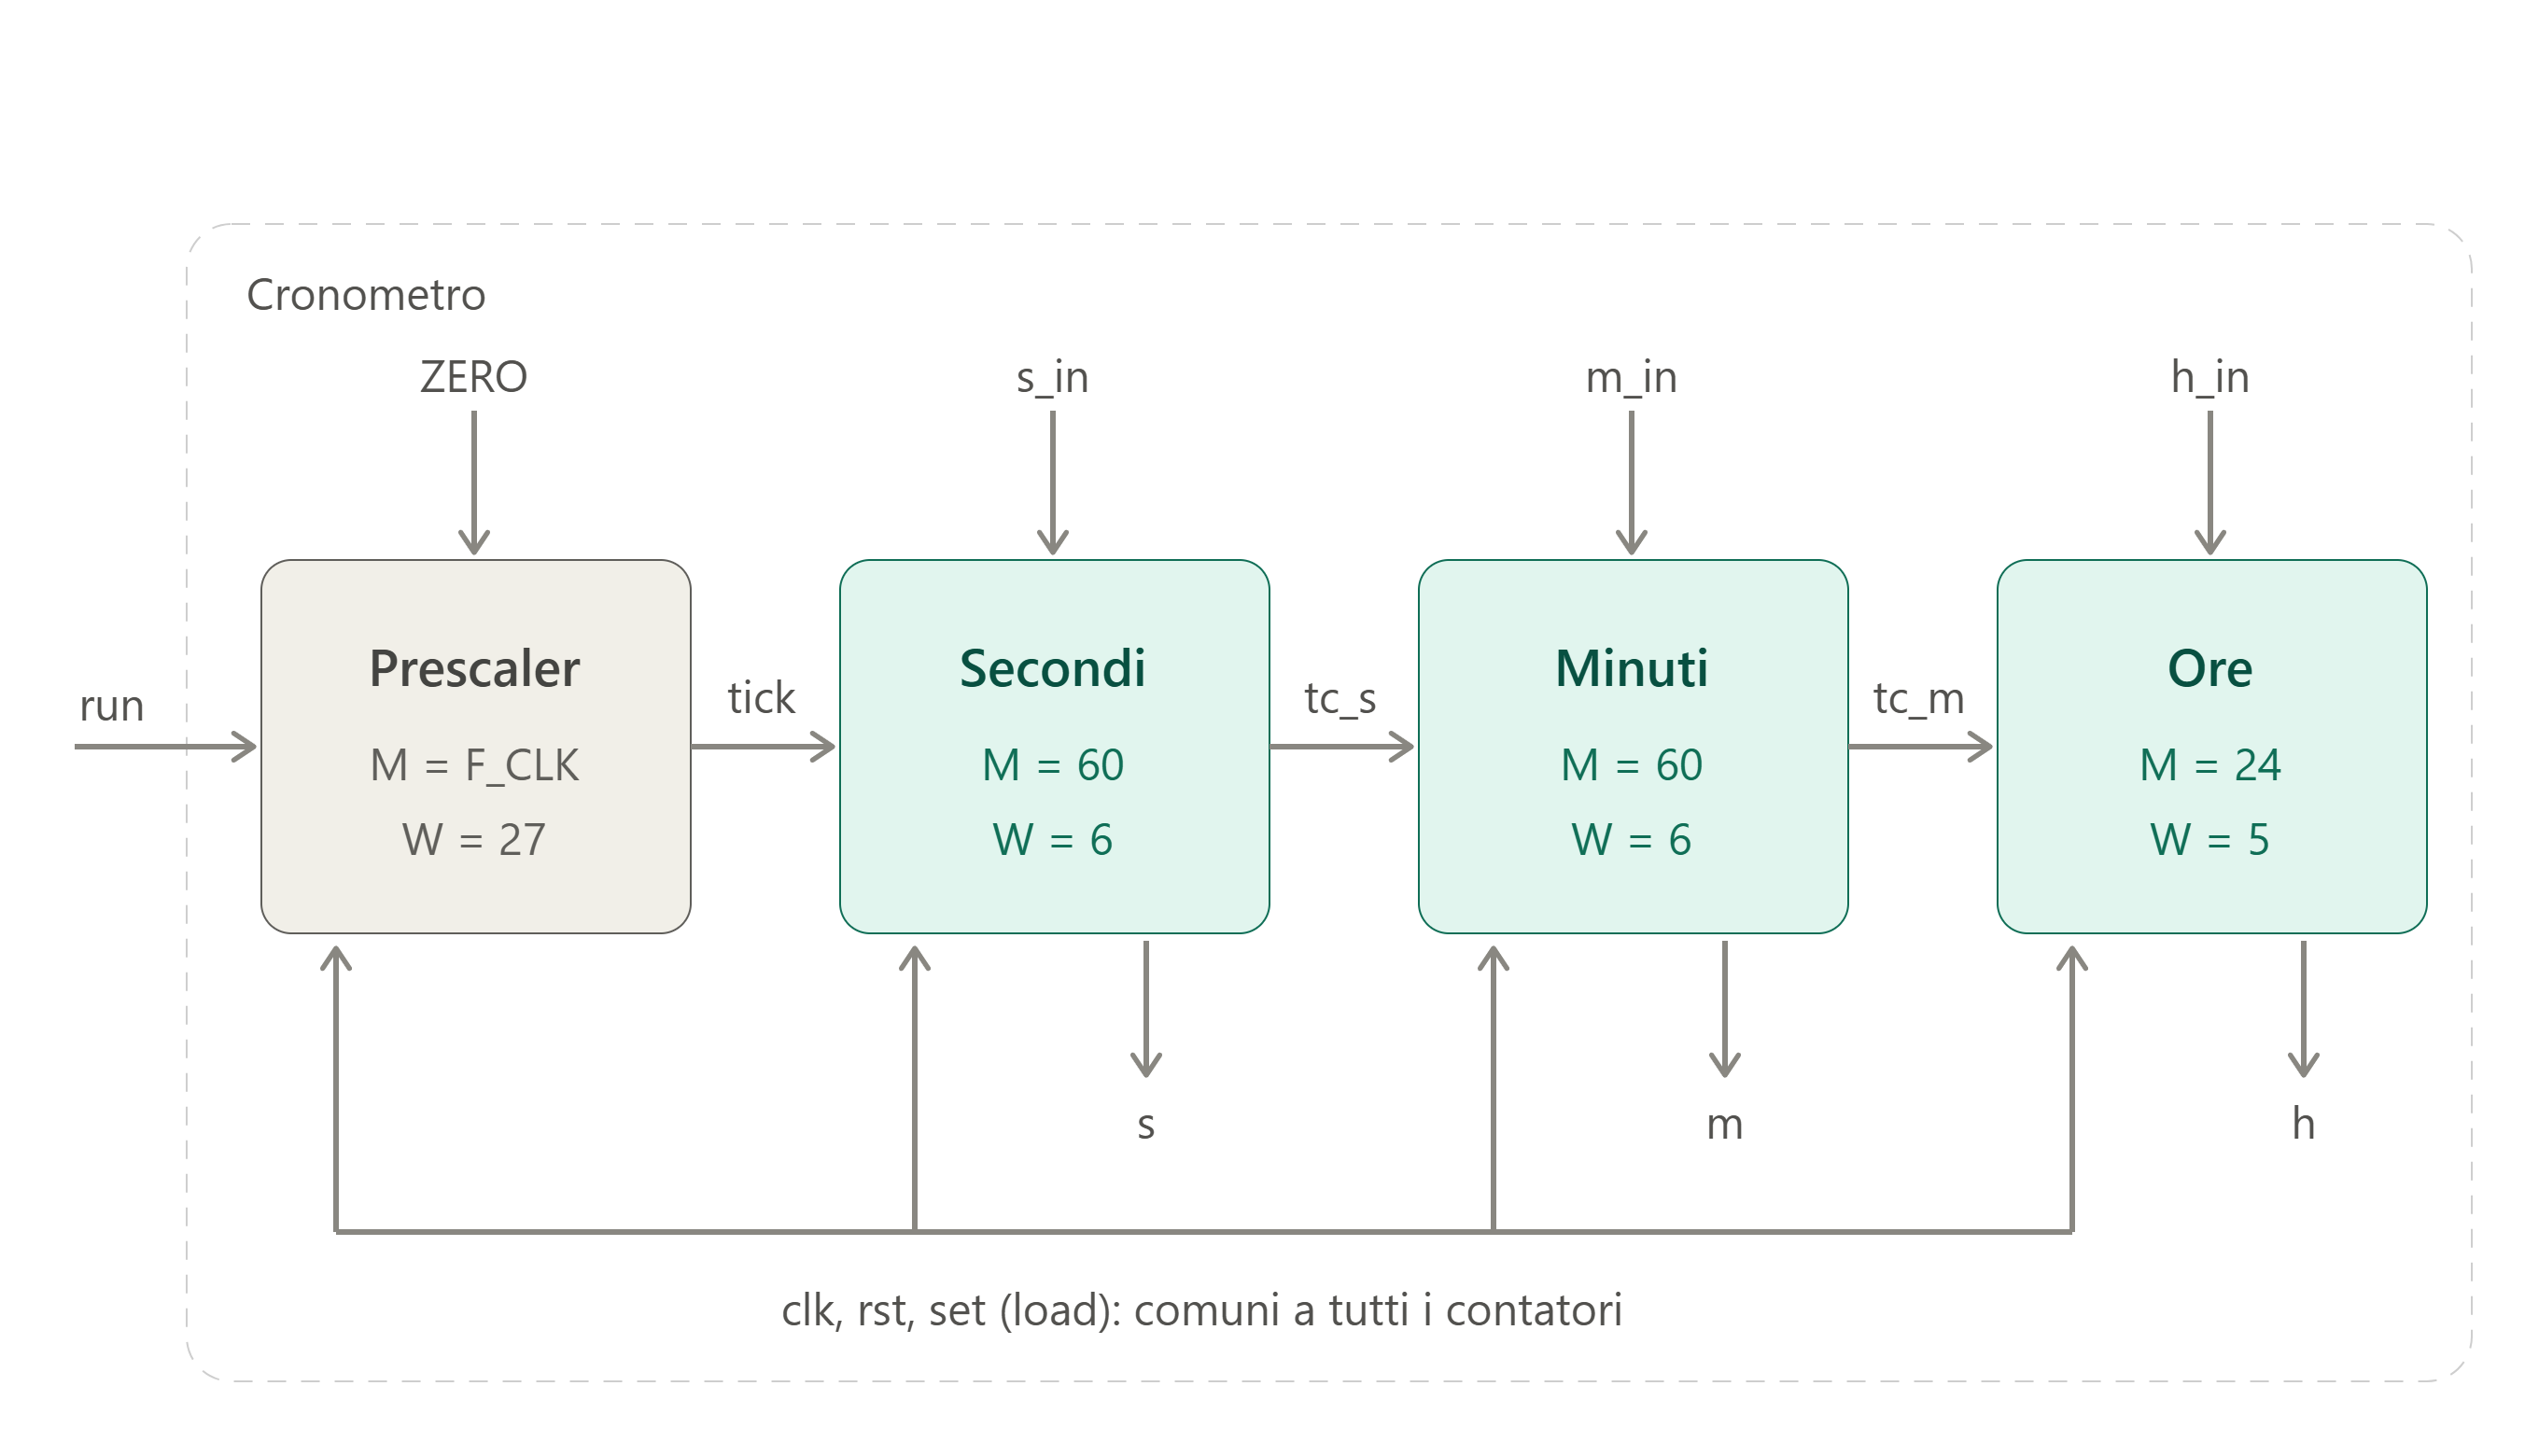
\includegraphics[width=0.7\linewidth]{figure/esercizio5-1/schema}
  \caption{Architettura del Cronometro}
  \label{fig:esercizio5-1:schema}
\end{figure}

Il valore iniziale è caricato tramite l'ingresso \texttt{load} dei contatori, collegato a \texttt{set}: ogni contatore riceve la propria parte del valore (\texttt{s\_in}, \texttt{m\_in}, \texttt{h\_in}), mentre il prescaler carica una costante nulla, così da ripartire dall'inizio del secondo.


\implementazione

Presentiamo per primo il contatore modulare \texttt{counter\_mod}, componente comune. I generic sono \texttt{M}, il modulo, e \texttt{W}, il numero di bit dell'uscita. Le porte sono \texttt{clk}, \texttt{rst} (reset sincrono), \texttt{en} (abilitazione al conteggio), \texttt{load} (caricamento del valore \texttt{d}), il dato \texttt{d} e l'uscita \texttt{q} a \texttt{W} bit, e infine il riporto \texttt{tc}. L'architettura è \texttt{behavioral}: un solo process sensibile a \texttt{clk} aggiorna il segnale interno \texttt{cnt}, con priorità decrescente a reset, caricamento e incremento; al raggiungimento di \texttt{M-1} il conteggio riparte da zero. Un \texttt{assert} con severità \texttt{failure} segnala il caso in cui \texttt{M} non è rappresentabile su \texttt{W} bit. Il riporto \texttt{tc} vale \texttt{'1'} quando \texttt{en} è attivo e il conteggio è a \texttt{M-1}, ossia quando al fronte successivo il contatore si azzera.

\vhdlfile{esercizio5-1/counter_mod.vhd}{Implementazione del Contatore modulare}{lst:esercizio5-1:counter-mod}

Definito tale componente, si riporta il top module \texttt{cronometro}. Il generic \texttt{F\_CLK}, di default 100\,000\,000, è il numero di cicli di clock per secondo. Le porte sono \texttt{clk}, \texttt{rst}, \texttt{run}, \texttt{set}, gli ingressi di inizializzazione \texttt{h\_in} (5 bit), \texttt{m\_in} e \texttt{s\_in} (6 bit) e le uscite \texttt{h}, \texttt{m}, \texttt{s} con le stesse larghezze. L'architettura è \texttt{structural}: la costante \texttt{W\_PRESC}, pari a 27, dimensiona il prescaler perché $2^{27}$ supera 100\,000\,000, mentre i segnali \texttt{tick}, \texttt{tc\_s} e \texttt{tc\_m} realizzano la cascata. Le quattro istanze \texttt{presc}, \texttt{sec}, \texttt{min} e \texttt{ore} sono create con port mapping e generic map; l'uscita \texttt{q} del prescaler e il riporto delle ore non sono utilizzati (\texttt{open}).

\vhdlfile{esercizio5-1/cronometro.vhd}{Implementazione del Cronometro}{lst:esercizio5-1:cronometro}

\simulazione

Il testbench \texttt{cronometro\_tb} ha entità senza porte e istanzia il top module come \texttt{dut}. Ai fini della simulazione \texttt{F\_CLK} è posto a 4: con un clock di periodo \texttt{T} di \SI{10}{ns}, un secondo corrisponde a \texttt{SEC} $= 4T = \SI{40}{ns}$. Il process \texttt{clk\_proc} genera il clock e \texttt{stim} applica la sequenza di stimoli, riportata di seguito.

\vhdlfile{esercizio5-1/cronometro_tb.vhd}{Testbench del Cronometro}{lst:esercizio5-1:cronometro-tb}

I passi del test sono i seguenti.
\begin{enumerate}
  \item Reset per due periodi di clock, poi \texttt{run} a \texttt{'1'} per cinque secondi: il tempo passa da 00:00:00 a 00:00:05.
  \item \texttt{run} a \texttt{'0'} per tre secondi: il conteggio resta fermo.
  \item Caricamento di 00:00:58 con un impulso di \texttt{set} e tre secondi di conteggio, fino a 00:01:00.
  \item Caricamento di 00:59:58, per verificare il riporto sulle ore (01:00:00).
  \item Caricamento di 23:59:58, per verificare il ritorno a 00:00:00 dopo 23:59:59.
  \item Impulso di \texttt{rst} e altri due secondi di conteggio.
\end{enumerate}

Il risultato della simulazione è mostrato in figura~\ref{fig:esercizio5-1:simulazione}.

\begin{figure}[H]
  \centering
  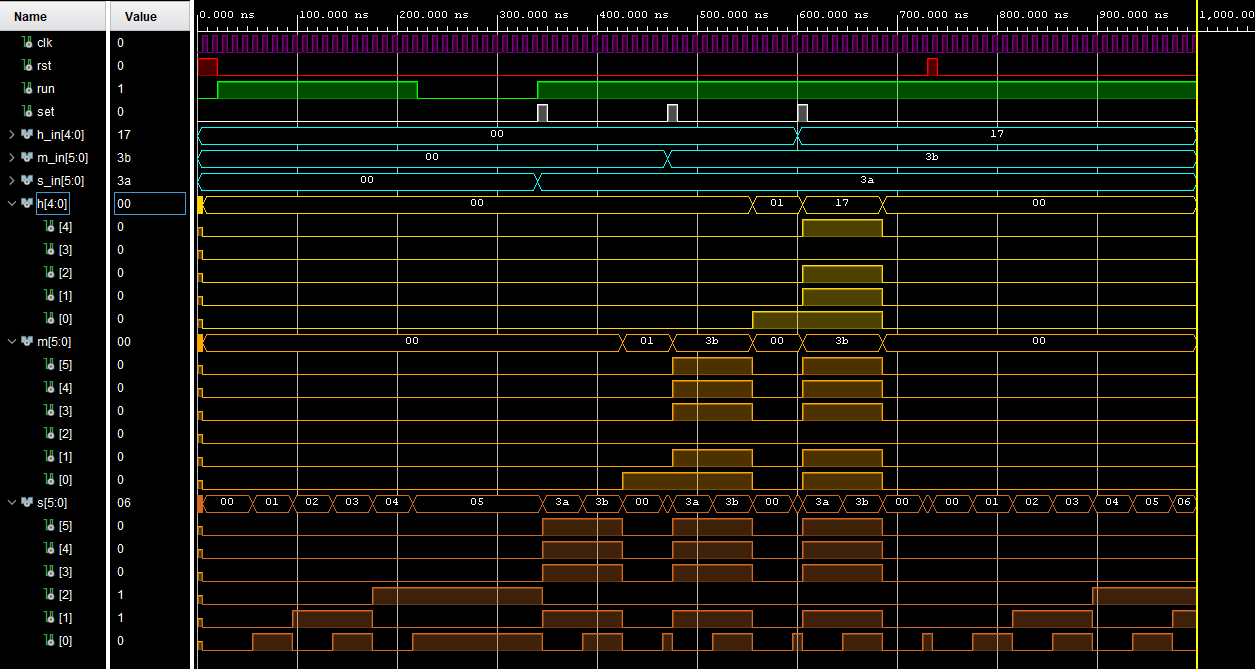
\includegraphics[width=\linewidth]{figure/esercizio5-1/simulazione}
  \caption{Simulazione del Cronometro}
  \label{fig:esercizio5-1:simulazione}
\end{figure}

Consideriamo il caricamento di 23:59:58. Con \texttt{h\_in} $=$ 0x17 ($10111_2$, ossia $23_{10}$), \texttt{m\_in} $=$ 0x3B ($59_{10}$) e \texttt{s\_in} $=$ 0x3A ($58_{10}$), un impulso di \texttt{set} porta le uscite a \texttt{h} $=$ 17, \texttt{m} $=$ 3b, \texttt{s} $=$ 3a. Dopo un secondo \texttt{s} vale 3b (59), dopo un altro secondo si azzera e il riporto propaga l'azzeramento a \texttt{m} e a \texttt{h}: le uscite tornano a 00:00:00. Nel caricamento precedente (00:59:58) l'ora passa da 00 a 01 e i minuti da 3b a 00. Dopo l'impulso di \texttt{rst} tutte le uscite sono a zero e il conteggio riprende dai secondi, che nell'ultima parte della figura arrivano a 06.

\begin{risultato}
La simulazione verifica il comportamento alle transizioni critiche (cambio di minuto, ora, giorno), l'arresto quando \texttt{run} è inattivo e l'azzeramento con \texttt{rst}.
\end{risultato}
